% Chapter Template

\chapter{Non-thermal emission from compact object merger} % Main chapter title

\label{ch:afg} % Change X to a consecutive number; for referencing this chapter elsewhere, use \ref{ChapterX}


\section{$\gamma$-ray bursts}

\acp{GRB} are irregular pulses of gamma-ray radiation with broken power-law (non-thermal) spectrum, peaking at KeV-MeV \citep{Band:1993,Kouveliotou:1993,Meegan:1992xg}.

With respect to the duration, \ac{GRB} are split into two categories: \ac{SGRB}, that last $< \sim 2$~s and long \ac{GRB} that last $> \sim 2$~s. The latter are the result of the collapse of massive $\geq 15M_{\odot}$ stars, while the former, at least in part, is attributed to mergers of compact objects. Only very recently it was directly confirmed \citep{TheLIGOScientific:2017qsa}. However, the exact physical origin of different duration \ac{GRB} is not fully understood.

Indications that long \ac{GRB} are associated with core-collapse supernovae, \acp{SN}, are two fold. These \acp{GRB} are typically observed in star-forming regions of their host galaxies \citep[\eg][]{Bloom:2000pq,Bloom:2002hc,Fruchter:2006py,Christensen:2004yx,CastroCeron:2006jh} and several \acp{GRB} are spectroscopically associated with Type Ic \acp{SN}, albeit these \acp{GRB} were significantly less bright and might not be typical \acp{GRB} \citep[\eg][]{Liang:2006ci,Bromberg:2011fm}. Additionally, the late time behaviour of some \acp{GRB} includes a \acp{SN}-like "bump" in the optical and spectral changes that might imply that underlying \acp{SN} flux becomes dominant over \acp{GRB} \citep[\eg][]{Bloom:1999,Woosley:2006fn}.

The \acp{GRB} are distant events, most of which were localized to outside the local group \citep[\eg][]{Mao:1992,Piran:1992,Fenimore:1993}. Particularly useful for distance estimation were the observations of \ac{GRB} afterglow, fading X-ray \& optical emission, that allow to estimate the redshift
\citep[\eg][]{Costa:1997cg,Frontera:1997ae}.

Analysis of the multi-wavelength afterglow data for \acp{GRB} \cite[\eg][]{Panaitescu:2001bx} suggested the mechanism behind the afterglow emission is the synchrotron radiation from the forward, external forward-shock, which forms when \ac{GRB}-ejecta sweeps-up the circumburst medium
\footnote{The specific indications are the power law decay of the light curves, $F_{\nu}\propto^{-1}$ and power-law spectrum $F_{\nu}\propto\nu^{-0.9\pm 0.5}$.} 
\citep{Rees:1992ek,Paczynski:1993gz,Meszaros:1993ju,Meszaros:1996sv}.

The temporal behavior of many (but not all) \acp{GRB} shows a change, a steepening of the light-curve (to $F_{\nu}\propto t^{-2.2}$) at $\sim 1$~day after the burst. This is usually attributed to the 
%\gray{deceleration of the colimated GRB-outflow, jet, and decrease on the realtivisitc beaming. This in turn makes the edge of the jet visible to an observer.} 
finite angular extend of the \ac{GRB}-ejecta, jet \citep[\eg][]{Rhoads:1999wm,Sari:1999mr}. When jet decelerates and relativistic beaming decreases (and the jet edge becomes visible), the optical and X-ray lightcurves decay achromatically faster. This achromatic transition from slow to faster decay is called "jet-break".

%% PROBLEMO -- jet-break is not a universal feature.
Notably, this jet-break is not observed in all GRBs which presents a question why \citep[\eg][]{Fan:2006pj,Panaitescu:2006,Liang:2007ti,Sato:2006jg,Liang:2007rn,Curran:2007cp,Racusin:2008bx}

%% PROBLEMO -- GRB density seems uniform, but SSE models predict wind-like profile
Models of the broadband emission of \acp{GRB} with jet-break showed that the circomburst medium, \ac{CBM}, is uniform with number density \red{$\sim 10^{-3}$} \citep{Panaitescu:2001bx}. If \acp{GRB} produced in collapse of massive stars \citep{Woosley:1993,Paczynski:1997yg}, this contradicts the expected density profile from stellar winds, \eg, $\rho\propto r^{-2}$ \citep[\eg][]{Dai:1998iz, Chevalier:1999jy, Chevalier:1999mi,Ramirez-Ruiz:2001} \red{this might be very outdated.}

%% sGRB
Regarding the short duration \ac{GRB}. Their origin was first connected with the elliptical galaxes with older stellar population \citep[\eg][]{Gehrels:2005qk,Fox:2005kv,Barthelmy:2005bx,Berger:2005dr,Panaitescu:2005er,Bloom:2005qx,Guetta:2005bb,Nakar:2007yr} and thus with merger of neutrons stars. A more direct evidence came with the detection of \GRB{} \cite{Abbott:2018wiz}, a \ac{SGRB} that accombaned the \ac{GW} detection and \ac{kN}.

Continuous observations of \ac{SGRB} showed a complex time behavior of early afterglow X-ray emission, in particular a presence of a plateau ($F_{x}\propto t^{-1/2}$), after the initial sharp decrease ($F_{x}\propto t^{-3}$) which a standard forward shock model does not predict. This implied that early X-ray afterglow is shaped by a variety of physical processes \citep{Zhang:2005fa}.

Two main questions that stem from these observations: is the mechanism behind the prompt $\gamma$-ray emission and early afterglow emission is the same (or do they originate from the same outflow), and is the early X-ray radiation produced by the external shock (just a blast wave takes long time to become self-similar) or does it originate from an internal shock?
An indication that the long-lived central engine activity might affect the afterglow came from the observed sharp increase in X-ray flux (flares) on a scale of minutes to hours after the end of the \ac{GRB}
\citep{Burrows:2005ww,Chincarini:2007fp,Chincarini:2010,Margutti:2011}, which could not be attributed to the inhomogeneities in the \ac{CBM}.
%% PROBLEMO!
Thus, the early X-ray behaviour of \acp{GRB} $t < 10^{4}$~s post-burst is not well understood and seems to be in tension with standard afterglow forward shock emission model.

%\textcolor{red}{
%    One of the foremost unanswered questions about GRBs is the physical mechanism
%    by which prompt $\gamma$-rays the radiation that triggers detectors on board
%    GRB satellites are produced. Is the mechanism the popular internal shock
%    model 6 \cite{(Rees and Meszaros, 1994)}, the external shock model, or something
%    entirely different? Are $\gamma$-ray photons generated via the synchrotron process
%    or inverse-Compton process, or by a different mechanism? Answers to these
%    questions will help us address some of the most important unsolved problems
%    in GRBs  how is the explosion powered in these bursts? Does the relativistic
%    jet produced in these explosions consist of ordinary baryonic matter, electron positron
%    pairs, or is the energy primarily in magnetic fields?
%}

Once again, while it is suggested that the high energy emission, after the propmt phase is produced by the synchrotron process in the external forward shock, \citep{Kumar:2009,Ghisellini:2010}, the mechanism behind the high and low energy $\gamma$-ray emission in the prompt phase remains unknown. 
Possible mechanisms include: inverse Compton and synchrotron emission in internal and external shocks
\citep[\eg][]{Rees:1992ek,Dermer:1998py,Lyutikov:2003ih,Zhang:2011} and 
photospheric radiation with contribution from multiple \ac{IC} scatterings
\citep[\eg][]{Thompson:1994zh,Ghisellini:1998jy,Meszaros:1999gb,Peer:2005qoc,Peer:2008udu,Giannios:2006jb,Ioka:2007qk,Asano:2009gi,Lazzati:2010,Beloborodov:2010,Toma:2011}.



\subsection{kilonova afterglow}

In addition to the \ac{GRB} beamed emission, the non-thermal, more isotropic emission is expected from electrons accelerated in shocks formed between the (mildly) relativistic ejecta and the \ac{ISM} \citep{Nakar:2011cw}. This emission is expected to peak in radio band and continue on a time scale of tens of years after merger. Notably, all ejecta components will contribute to the emission, but  depending on the ejecta velocities and kinetic energy, the brightness in different frequencies and timescales differs. 

Various ejecta components interact with each other and with \ac{ISM}. The latter, generates a long-lived blast wave. The shock, propagating upstream, amplifies (random) magnetic fields and accelerates electrons, that subsequently emit synchrotron radiation. This process in phenomenological similar to the for the \ac{GRB} afterglow and \ac{SN} early remnants. 

\red{There is not much intro I found here, maybe because it has never been observed before}



\section{Theoretical background}

This section aims to outline a brief overview of the most relevant physical processes in GRBs. Tt is not meant as a comprehensive theoretical review. For this we refer the interested reader to the momnograph by \citet{RybickiLightman:1985}, as well as books of high energy astrophysics by \citet{Longair:2011,Dermer:2009}.

In this section we focus first on certain aspects of theory of special relativity, and relativistic hydrodynamics 
\red{this is where you put the NAVA and Peer models for dynamcs, Sedov Teylor and stuff maybe 
and on radiation processes, synchrotron, \red{inverse-Compton} and \red{photon-pion} processes.
}


\subsection{Special relativistic effects}

\begin{figure*}[t]
    \centering 
    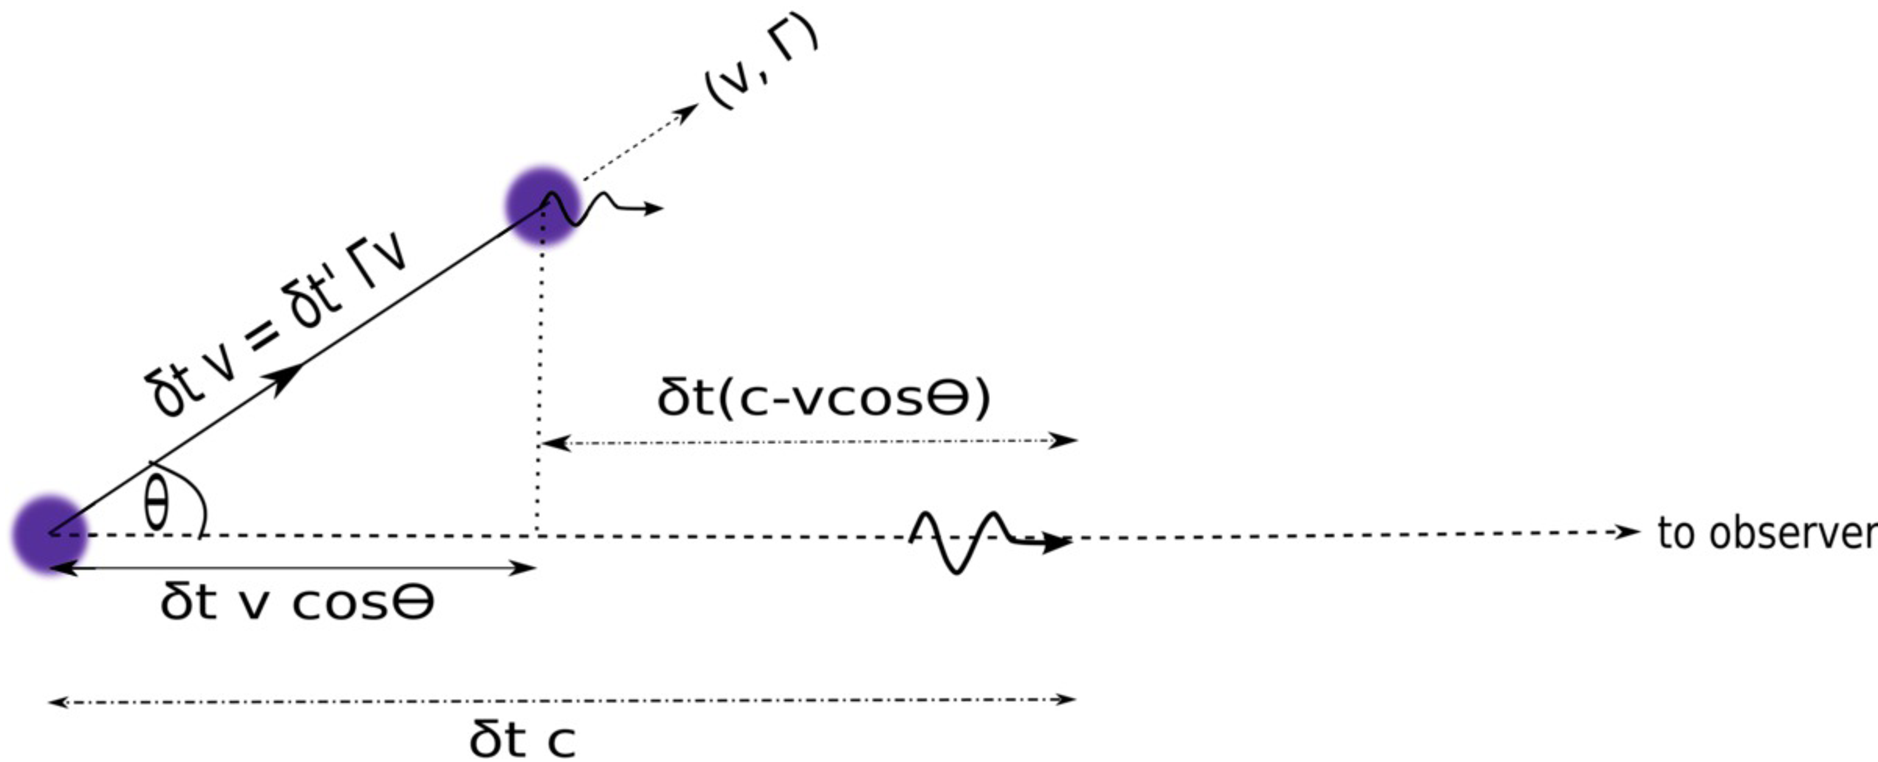
\includegraphics[width=0.45\textwidth]{Fig_1_KZ.pdf}
    \caption{
        The relation between pulse duration in source comoving frame, $\delta t'$, lab frame
        $(\delta t)$, and the time interval for pulse received by a distant observer is shown in this
        gure. The source is moving with speed $\upsilon$ (Lorentz factor $\Gamma$), at an angle $\theta$ with
        respect to observer line of sight. One photon is emitted when the source was at the
        location at the left side of the gure. And a second photon is emitted $\delta t'$ later when
        the photon has already traveled a distance ct toward the observer, and the source
        is also a distance $\upsilon$ cos $\theta\delta t$ closer. The dierence between these two distances is the
        time interval in the observer frame for the arrival of the two photons which is given
        by equation 1.
        (Adapted from \citet{Kumar:2014upa}, Fig.~1)
    }
    \label{fig:aafg:theory:sr1}
\end{figure*}

Consider a moving source of radiation and an observer with a line of sight to the source. Let $\upsilon$, $\Gamma$ and $\theta$ be the source velocity, \ac{LF} and angle with the line of sight. \red{REPLACE $\theta$ with $\Phi$ for consistency! (remember spreading jet)}

Consider three frames of reference, the comoving frame (usually denoted with a prime $'$), the lab frame, where the source is seen as moving with $\upsilon$ and observer frame. Then, if two photons are emitted in the comoving frame with time difference of $\delta t'$, which is in the lab frame $\delta t = \Gamma \delta t'$, the observer sees the two photons arrive with 

\begin{eqnarray}
\delta t_{obs} &= \delta t + \frac{(d - \upsilon\cos(\theta) \delta t)}{c} - \frac{d}{c} \\
&= \delta t (1 - \upsilon \cos(\theta) / c) \\
&= \delta t' \Gamma (1 - \upsilon \cos(\theta) / c)\\
&= \delta t' \mathcal{D}^{-1}
\end{eqnarray}

where $d$ is the distance to the source, and 

\begin{equation}
\mathcal{D} = \frac{1}{\Gamma(1 - (\upsilon/c) \cos(\theta))} = \frac{1}{\Gamma(1 - \beta\cos(\theta))}
\end{equation}

is the \ac{DF}. 
\gray{Note that if $\theta \ll 1$ and $\Gamma \gg 1$, the $\delta t_{obs} \approx (\delta t' / \Gamma) (1 + \theta^2 \Gamma^2)/2 = (\delta/\Gamma^2)(1 + (\theta\Gamma)^2/2)$}.
See Fig.~\ref{fig:aafg:theory:sr1}.

Next, we consider the transformation of the photon frequencies. 
Once again $\nu'$ denotes the frequency in the comoving frame and $\nu$ denotes the frequency in the observer frame. 
We employ the standard Lorentz transformation of the photon $4$-momentum in comoving frame, \eg,, $\nu'(1, \cos(\theta'), \sin(\theta'),0)$ to the lab frame $4$-momentum $\nu(1, \cos(\theta), \sin(\theta), 0)$

\begin{equation}
\nu = \nu' \Gamma(1+\upsilon \cos(\theta')/c) \text{ \& } \nu\cos(\theta) = \nu' \Gamma (\cos(\theta') + \upsilon/c)
\end{equation}

or 

\begin{equation}
\nu = \frac{\nu'}{\Gamma (1 - \upsilon\cos(\theta)/c)} = \nu' / \mathcal{D}
\end{equation}

which is a standard Doppler shift formula.
\red{This formula is used in the Code to convert given frequency into the comoving one}


\subsubsection{Relativistic beaming of photons}

We have shown that $\nu = \nu' \mathcal{D}$, but also $\sin(\theta) = \sin(\theta')/\mathcal{D}$. Then the transverse component of the momentum is invariant under the Lorentz transformation, \eg, $\nu_{\perp}' = \nu'\sin(\theta') = \nu\sin(\theta) \nu_{\perp}$. 
For a beem of photons it imples that the angular size of the beem is smaller in the lab frame than in the comoving frame by $\propto \Gamma$.
The solid angle of a conical beem of photons, $d\Gamma$ then 

\begin{equation}
d\Gamma = \sin(\theta)d\theta d\phi = \sin(\theta') d\theta' d\phi' / \mathcal{D}^2 = d\Omega'/\mathcal{D}^2
\end{equation}

is smaller in the lab frame than in the comoving frame.

Next, consider a frequency integrated total energy radiated per init time over the $4\pi$ steradians, denoted as $P$. 
\gray{Assume that the photon been is symmetric under the parity transformation in particle rest-frame (energy radiated per unit of the solid angle in $\theta\phi$ and $\pi-\theta,\pi+\phi$ are the same} \red{assume emission is locally isotropic.}.
%% ---
The the power in the lab frame $P = P'\Gamma\delta t'/(\Gamma\delta t') = P'$. 
Hence, power radiated by particles is \magenta{Lorentz invariant}.


\subsubsection{Transformation of specific luminosity and specific intensity}

Consider a spherically symmetric source, expanding with Lorentz factor $\Gamma$. 
%% ---
Introduce the \magenta{specific luminosity}, defined as the total energy that passes through the surface enclosing the source per unit time, per unit frequency, $L_{\nu} = dE / d\nu dt_{obs}$. 
As $d\nu dt_{obs} = d\nu' dt'$ and $E=\Gamma E'$, the Lorentz transformation of luminosity is

\begin{equation}
L_{\nu} = \frac{dE}{d\nu dt_{obs}} = \Gamma \frac{dE'}{d\nu' dt'} = \Gamma L_{\nu}'
\end{equation}

assuming that the $3$-momentum is zero (as the source is spherically symmetric).

Next, introduce the \magenta{specific intensity}, defined as a flux per unit frequency and per unit solid angle, mediated by photons, transversing surface $dA$, perpendicular to the conical beam, confining the photons, 

\begin{equation}
I_{\nu} = \frac{dE}{d\nu dt_{obs} dA d\Omega}
\end{equation}

that has a Lorentz transformation $I_{\nu} = \mathcal{D}^3 I_{\nu'}'$ as $d\nu dt_{obs} dA$ is the Lorentz invariant.


\subsubsection{Observed \ac{LC} from a source that is suddenly turned off}

\begin{figure*}[t]
    \centering 
    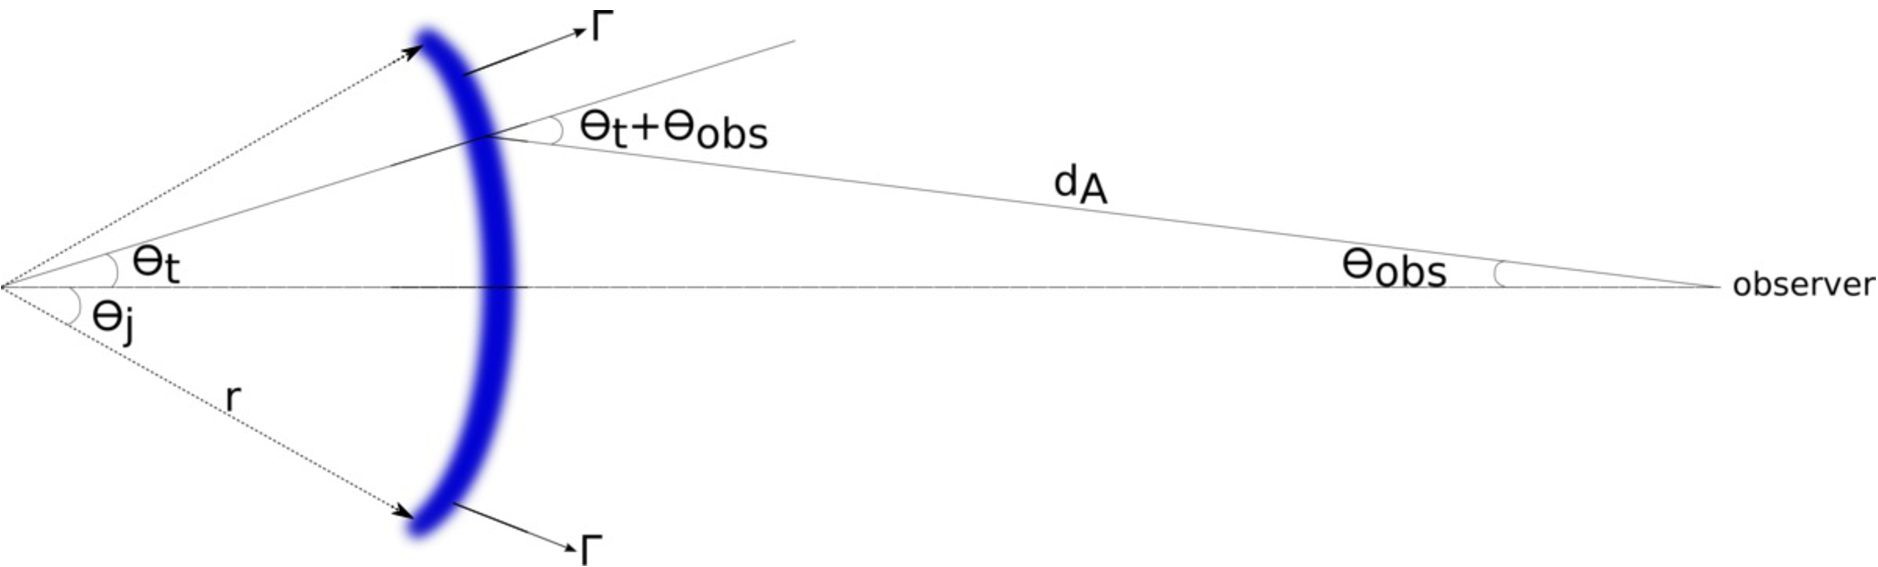
\includegraphics[width=0.45\textwidth]{Fig_2_KZ.pdf}
    \caption{
        The relation between pulse duration in source comoving frame, $\delta t'$, lab frame
        $(\delta t)$, and the time interval for pulse received by a distant observer is shown in this
        gure. The source is moving with speed $\upsilon$ (Lorentz factor $\Gamma$), at an angle $\theta$ with
        respect to observer line of sight. One photon is emitted when the source was at the
        location at the left side of the gure. And a second photon is emitted $\delta t'$ later when
        the photon has already traveled a distance ct toward the observer, and the source
        is also a distance $\upsilon$ cos $\theta\delta t$ closer. The dierence between these two distances is the
        time interval in the observer frame for the arrival of the two photons which is given
        by equation 1.
        (Adapted from \citet{Kumar:2014upa}, Fig.~1)
    }
    \label{fig:aafg:theory:sr2}
\end{figure*}

\red{it mainly says that when the source turns off, because of its finite angular extend and EATS, the observed flux does not switches off, but rapidly declies.}

Considering the variability of \ac{EM} transients such as \ac{GRB} it is important to asses how a sudden turn off of the source affects the observed emission. 
Consider a relativist thin shell moving within a cone with \ac{LF} $\Gamma$. As it reaches the radius $r=R_0$ the source turns off. 
\red{
    A point on the thin shell is characterized by $(r,\theta,\phi)$ where $\theta$ is the angle measured with respect to the line of sight to the observer. Then, photons, emitted at $(r=\upsilon t, \theta,\phi)$ arrive at the observer with a time delay with respect to a photon emitted at $r=0$ of
}

\begin{equation}
t_{obs} = t - \frac{r \cos(\theta)}{c} = t(1-\frac{\upsilon\cos(\theta)}{c}) = \frac{t}{\Gamma\mathcal{D}}
\end{equation}

Now, consider the observed emission from the source at frequency $\nu$. The starting time is $t_{0;obs}\approx(R_02c\Gamma^2)$, at which photons, emitted from $(R_0,0,0)$ arrive, At later times, $t_{obs}>t_{0;obs}$, the observer still sees photons emitted when $r < R_0$. 
Assume that the intrinsic emission spectrum is $I_{\nu'}' = I'\nu^{'-\beta}$.
Then, at $t_{obs} > t_{0;obs}$ the radiation from $\theta > \theta_t$ (where $\theta_t$ corresponds to $t_{obs} = R_0(1/\upsilon - \cos(\theta_t)/c)$) reaches the observer.
The observed flux \eg, $f_{\nu} \propto \int I_{\nu} d\Omega$, has the following Lorentz transformation $f_{\nu}\propto\int_{\theta_t} d\theta \sin(\theta_t) \mathcal{D}^{-(3+\beta)}$.

Now, consider a more rigorous derivation of the transformation of the specific flux in observer frame from relativistic source with comoving specific intensity $I_{\nu'}'$ and spectrum $\propto \nu^{' -\beta}$

\begin{equation}
f_{\nu}(t_{obs}) = \int d\Omega_{obs} I_{\nu} \cos(\theta_{obs}) = 2\pi \int d\theta_{obs} \frac{ I_{\nu'_0}' \nu_{0}^{'\beta}\sin(2\theta_{obs})[(1+z)\Gamma]^{-(3+\beta)} }{ 2\nu^{\beta} [ 1-\upsilon\cos(\theta + \theta_{obs}) / c ]^{3+\beta} }
\end{equation}

where $\nu_0 '$ is a frequency that lies on the power law segment of the spectrum for $I_{\nu'}'$. The Lorentz transformation of the specific intensity was made above. The factor $(1+z)^{3+\beta}$ accounts for the Redshift on the frequency. 

Assuming that $\sin(\theta)/d_{A} = \sin(\theta_{obs})/r$, the above integral writes 

\begin{equation}
f_{\nu} \approx \frac{ 2\pi I' \nu' _0 \nu_{0}^{'\beta}\nu^{-\beta} }{[(1+z)\Gamma]^{3+\beta}} \Big( \frac{R_0}{d_A} \Big)^2 \int_{\theta_t}^{\pi / 2} d\theta \frac{\sin(\theta)\cos(\theta)}{(1-\upsilon\cos(\theta)/c)^{3+\beta}},
\end{equation}

where $\theta+\theta_{obs}$ in the denominator was replaced with $\theta$ as $\theta_{obs}\ll\theta$.
The integral is simple to compute. Ir yields

\begin{equation}
f_{\nu}(t_{obs}) \propto (1 - \upsilon\cos(\theta_t)/c)^{-(2 + \beta)}\nu^{-\beta} \propto t_{obs}^{-(2+\beta)} \nu^{-\beta},
\end{equation}

This equation shows, that the observed radiation does not immediately turns off when the source switches off. The flux falls off rapidly with time and vanishes when $\theta_t$ exceeds the angular size of the source $(\theta_j)$.


\subsection{Synchrotron Radiation}

\red{This is not exactly accurate formalism, does not take angle into account}
\red{Could be considerably imprved}

Consider an electron moving in the magnetic field, perpendicular to the field lines.
Let $\gamma_e$, $\upsilon_e$ be the electron's \ac{LF} and velocity and $B$ the magnetic field strength.
The electric field in the electron rest-frame is $E=\gamma_e \upsilon_e B /c$. The electron acceleration in this field yields radiation, total power of which, according to the Larmor's formula, 

\begin{equation}
P_{syn} = \frac{2q^4E^2}{3c^3m_e}=\frac{2q^4B^2\gamma_e^2\upsilon_e^2}{3c^5m_e^2}=\frac{\sigma_TB^2\gamma_e^2\upsilon_e^2}{4\pi c}
\end{equation}

where $\sigma_T = 8\pi q^4 / (3m_e^2c^4)$ is the Thompson cross section. 

The $P_{syn}$ is the Lorentz invariant (as electric dipole radiation is Lorentz invariant).

Note, that for an isotropic pitch angle distribution, the average power $\langle P_{syn} \rangle = (2/3)P_{syn}$.

The angular speed of the electron (\eg its Larmor frequency), is

\begin{equation}
\omega_L = \frac{q B}{\gamma_e m_e c}
\end{equation}

\red{nice rephrasing}
Within the magnetic field, an electron is moving on a spiral trajectory. 
The relativistic beaming of emitted radiation leads to a distant observer being able to see this radiation, only when the electron velocity vector is within $\angle \sim \gamma_e^{-1}$ from the lшne of sight. Correspondingly, only a fraction of orbital time, $t\sim1/(\pi\gamma_e)$, contributes to the observed radiation, which appears as a repeated pulse. 
The duration of this pulse is

\begin{equation}
\delta t_{obs} \sim \frac{2}{\gamma_e \omega_L}\frac{1}{2\gamma_e^2}\sim \frac{m_e c}{q B \gamma_e^2}
\end{equation}

where we used $\delta t' = \delta t / \gamma_e$. 
Then the characteristic frequency of the synchtrontron radiation is given by an inverse of $\delta t$ and reads 

\begin{equation}
\omega_{syn} \sim \frac{q B \gamma_e^2}{m_e c} \text{ and } \nu_{syn} = \frac{\omega_{syn}}{2\pi} \sim \frac{q B \gamma_e^2}{2\pi m_e c}
\end{equation}

where $\nu_{syn}$ is the cyclic frequency.
Note that here the factor $(3/2)\sin(\alpha)$, where $\alpha$ is the pitch angle between the electron's velocity and the magnetic field is \red{ommited}.

The synchrotron spectrum peaks at $\sim \nu_{syn}$. At $\nu < \nu_{syn}$ the $P_{syn}(\nu)\propto\nu^{1/3}$ (which is determined by the Fourier transform of the synchrotron pulse profile). At $\nu > \nu_{syn}$ the power decays exponentially. See \citet{RybickiLightman:1985} for the calculation of synchrotron spectrum.

The power per unit frequency at the peak of the spectrum is given 

\begin{equation}
P_{syn}(\nu_{syn}) \sim \frac{P_{syn}}{\nu_{syn}} \sim \frac{\sigma_T B m_e c^2}{2 q},
\end{equation}

Now consider the distribution of electrons.
Commonly adopted is the power-law distribution, $dn_e/d\gamma_e \propto \gamma_e^{-p}$, which results in emission spectrum $f_{\nu}\propto\nu^{-(p-1)/2}$,
which is a consequence of 

\begin{equation}
f_{\nu} = \int_{\gamma_{\nu}}^{\infty} d\gamma_e \frac{dn_e}{d\gamma_e}P_{syn}(\nu) \propto \nu^{-(p-1)/2}
\end{equation}

as $P_{syn}(\nu) \propto (\nu/\nu_{syn})^{1/3}$ for $\nu < \nu_{syn}$\red{where is this from?}.

Here

\begin{equation}
\gamma_{\nu} \sim \Bigg(\frac{2\pi\nu m_e c}{qB}\Bigg)^{1/2}
\end{equation}

is the minimum \ac{LF}, above which electrons contribute to the specific flux, $f_{\nu}$
\red{why?}
\gray{This seems to be an equation for $\nu = f(\gamma)$ inverted, -- so is the $\nu$ a critical frequency?}



\subsubsection{Effect of synchrotron cooling on electron distribution}

Consider the effects of electrons cooling. 
The characteristic frequency associated with it is $\nu_c$ and \фсХДАЪ $\gamma_c$.
Electrons with \ac{LF} $\gamma_e > \gamma_c$ can efficiently loose their energy to synchrotron radiation. Then, after the time $t_0$, their $\gamma_e$ drops below $\gamma_c$, 

\begin{equation}
c^2 \frac{dm_e}{dt} \gamma_e = -\frac{\sigma_T}{6\pi} B^2 \gamma_e^2 c
\end{equation}

which result in 

\begin{equation}
\gamma_c \sim \frac{6 \pi m_e c}{\sigma_T B^2 t_0}
\end{equation}

The corresponding characteristic frequency is called the synchrotron cooling frequency

\begin{equation}
\nu_c = \frac{3}{4\pi} \gamma_c^2 \frac{q B}{m_e c}
\end{equation}

At $\nu_c$ the spectrum of the synchrotron radiation is changing, as electrons with $\gamma_e > \gamma_c$, the effects of cooling modify the electron distribution. 

Consider the continuity equation for electrons in the energy space 

\begin{equation}
\frac{\partial }{\partial t}\frac{d n_e}{d\gamma_e} + \frac{\partial}{\partial \gamma_e}\Big[ \dot{\gamma_e}\frac{dn_e}{d\gamma_e} \Big] = S(\gamma_e)
\end{equation}

where $\dot{\gamma_e} = -\sigma_T B^2 \gamma_e^2 / (6\pi m_e c)$ is the rate at which electron \ac{LF} changes due to losses, $S(\gamma_e)$ is the injection rate of electrons into the system.
%% ---
Assume that the minimum \ac{LF} of injected electrons is $\gamma_m$, \eg, where $S(\gamma_e) = 0$ for $\gamma_e < \gamma_m$.
Then if $\gamma_c < \gamma_e < \gamma_m$ the solution to the equation $dn_{e}/d\gamma_e \propto \dot{\gamma_e}^{-1} \propto \gamma_e^{-2}$.

Then, for this electron distibution the synchrotron spectrum is $f_{\nu}\propto\nu^{-1/2}$ 
\footnote{If $B=f(t)$, then the distribution function for $\gamma_e$ evolves with time and is not a simple pwoer law with index $2$, see \citet{Uhm:2013gwa}.}

For $\gamma_e > \gamma_c > \gamma_m$, the solution to the equation is $dn_e/d\gamma_e \propto \gamma_e^{-p-1}$ (assuming the constant $B$ field, the steady state). Then the synchrotron spectrum reads $f_{\nu}\propto\nu^{-p/2}$.


\subsubsection{Synchrotron self-absorption frequency}

If the photon absorption by the inverse-synchrotron process is important, another characteristic frequency, $\nu_a$, can be determined. Consider the Kirchhoff's law, \red{stating that the emergent specific flux cannot exceed the black-body flux corresponding to the appropriate electron temperature} which is

\begin{equation}
k_BT\approx \max(\gamma_a,\min[\gamma_m,\gamma_c])m_e c^2 / 2.7
\end{equation}

where $\gamma_m$, $\gamma_c$ and $\gamma_a$ are electron Lorentz factors corresponding to $\nu_m$, $\nu_c$ and $\nu_a$.
Then the \red{synchrotron self-absorption frequency $\nu_a$ is the frequency where the emergent synchrotron flux is equal to the black body flux}

\begin{equation}
\frac{2m_ec^2\max(\gamma_a,\min[\gamma_m,\gamma_c])\nu_a^2}{2.7c^2}\approx\frac{\sigma_T B m_e c^2 N_>}{4 \pi q}
\end{equation}

where the LHS is the Plank function in the Rayleigh-Jeans limit and $N_{>}$ is the column density of electrons with Lorentz factor larger then $\max(\gamma_a\min[\gamma_m,\gamma_c])$.

Finally, the order of characteristic frequencies determines the emergent synchrotron spectrum for a distribution of electrons. 
See Fig.X for fast and slow cooling regimes \citet{Sari:1997qe}.


\subsubsection{Synchrotron self-absorption via flux attenuation}

\red{To be written from Dermer+2009}


\subsubsection{Maximum energy of synchrotron photons}

Consider a shock front. Scattering back and forth, particles within it accelerate via the \magenta{first order Fermi process}, increasing their energy $\times 2$ times, at every front of the shock.
In order to determine what is the maximum energy a particle can reach consider the following. A charged particle of mass $m$ accelerates while crossing the shock front on a timescale $\sim$ Larmor time, $t'_L = mc\gamma/(qB')$, where primed quantities are measured in the rest frame of the fluid and $\gamma$, \ac{LF} on a particle in the frame, comoving with the shock. 
%% ---
The particle can accelerate to $\gamma$ only if it losses less then half of its energy to synchrotron emission in $t'_L$. Then 

\begin{equation}
\frac{4 q^4 B^{'2}\gamma^2 t'_L}{9 m^2 c^3} < \frac{m c^2\gamma}{2} \text{ or } \nu\propto \frac{q B' \gamma^2}{2\pi m c} < \frac{9 m c^3}{16\pi q^2}
\end{equation}

Thut, for electron the maximum synchrotron photon energy is $\sim 50$~MeV and for proton it is $\sim 100$~GeV in the shocked fluid comoving frame. \red{assuming Bohm diffusion limit.}
This limit can be exceeded in case of highly inhoogeneous magnetic field \citep{Kumar:2012}.


\subsubsection{Inverse-Compton radiation}

%% SINGLE electron, Single Photone
The \ac{IC} scattering is the scattering of photons by electrons of larger energy, resulting in increase in photon energy on average.
%% ---
Consider electrons with $\gamma_e$ and photons with frquency $\nu$. Let $h\nu\gamma_e \ll m_e c^2$. The average frequency of scattered photons then $\nu_s\sim\nu\gamma^2_e$.
\gray{
    This can be seen from considering the scattering in the rest frame of the electron.
    Let the incident photon have frequency $\nu' \sim \nu\gamma_e$. (See eq.for Doppler Shift). If $h\nu'\ll m_e c^2$, the scattering is elastic (electron recoil is negligible) and the post-scattering angle distribution is a dipol function. 
    Then, transforming the $\nu'$ into the original frame results in $\nu_s\sim\nu\gamma_e^2$.
}

%% Single electron, Radiation Field
Consider a radiation field with photon density $u_{\gamma}$, and an electron moving through it. 
Then, the power in \ac{IC}-scattered photons is (assuming $h\nu\gamma_e\ll m_e c^2$)

\begin{equation}
P_{ic} \sim \sigma_T \int d\nu \frac{u_{\nu} c}{h\nu} h\nu\gamma_e^2 \sim \sigma_T u_{\gamma}\gamma^2_e c;
\end{equation}

where $u_{\nu}d\nu$ is the energy density in photons of frequency between $\nu$ and $\nu+d\nu$, such $\int d\nu u_{\nu} = u_{\gamma}$. From $P_{sync}$ (see eq.above.somewhere) and this equation $P_{sync}/P_{IC} \sim u_{B}/u_{\gamma}$, where $u_{B}- B^2 / 8\pi$.

Now consider, that the radiation field is generated by the synchrotron process, \ie, photons are produced by and scattered on the same electrons (to typically much higher energies). This process is called \magenta{synchrotron-self-Compton} or \ac{SSC}.
The relative importance of \ac{IC} process is specified by the Compton paramter $Y$ for a population of energetic electrons. 
Consider an energy density in photons for synchrotron process

\begin{equation}
u_{\gamma} = \int dr \int d\gamma_e \frac{P_{syn}}{c}\frac{dn_e}{d\gamma_e} = \frac{\sigma_T (\delta R) B^2}{6\pi} \int d\gamma_e \gamma^2_e \frac{d n_e}{d\gamma_e} = \frac{\sigma (\delta R) n_e B^2}{6\pi}\langle\gamma_e^2\rangle
\end{equation}

where $\delta R$ is the radial width of the source, and 

\begin{equation}
\langle \gamma_c^2\rangle = \frac{1}{n_e} \int d\gamma_e \gamma_c^2\frac{dn_e}{d\gamma_e}.
\end{equation}

Invoking the formula \red{which} for the $u_{\gamma}$ for synchrotron radiation, the Compton parameter reads 

\begin{equation}
Y \sim P_{IC} / P_{syn} \text{ where } \tau_e = \sigma_T (\delta R) n_e
\end{equation}

is the optical depth of the source to Thompson scattering.

\paragraph{IC spectrum.}

In order to obtain IC radition spectrum, the seed photon spectrum is to be convolved with electron distribution \citep{RybickiLightman:1985}

\begin{equation}
f_{IC}(\nu_{IC}) \approx \frac{3\sigma_T (\delta_R)}{4} \int d\nu \frac{\nu_{IC}}{\nu^2}f_{syn}(\nu) \int \frac{d\gamma_e}{\gamma_e^2}\frac{dn_e}{d\gamma_e}F\big( \nu_{IC} / 4 \gamma_c^2\nu \big)
\end{equation}

where 

\begin{equation}
F(x) \approx \frac{2}{3}(1-x), \text{ and } x = \frac{\nu_{IC}}{4\gamma_e^2\nu}
\end{equation}

To qualitatively asses the spectrum, assume that the seed photon spectrum is a $\delta$-function around frequency $\nu_0$. Electron distribution is power law with index $p$.
%% ---
Consider the low energy side, where the spectrum is cut off at $\gamma_m$, is proportional to $\nu_{IC}$ for $\nu_{IC} < 4\gamma_m^2\nu_0$. Then, if \ac{SSA} is neglected, then the \ac{IC} spectrum at low energies is much steeper than the hardest synchrotron spectrum $\propto\nu^{1/3}$.
Now, consider the high energy side, $\nu_{IC} > 4 \gamma_m^2\nu_0$. There, the \ac{IC} spectrum approaches $\propto \nu_{IC}^{-(p-1)/2}$, same as the synchrotron process spectrum.

\paragraph{IC in Klein-Nishina regime}

The assumed non-elastic scattering of photons is only valid as long as photon energy is lower then $m_e c^2$ in the comoving frame. When this condition is not longer valid, the electron recoil in the scattering can no longer be ignored. Additioanlly, the cross-section becomes smaller then $\sigma_T$ (decreasing with rising photon energy). 
The electron recoil also leads the the change in upper limit of the scattered photon energy, $\sim m_e c^2 \gamma_e / 2$. See \citet{RybickiLightman:1985} for equations.


\subsubsection{Hadronc processes}
\red{very brief}

Under the hadronic processes one understands the followign processes.
The photon-pion process, \ie, the production of pions ($\pi^0, \pi^+$ and $\pi^-$), the decay of $\pi^+$ produces $p^+$ with high lorentz factor that can cool via synchrotron processes.
The Bethe-Heitler pair production process.
Others...

%% ====================================================
%%
%%               A F T O R G L O W
%%
%% ====================================================

\section{Afterglow Theory}

Consider a dynamics of a relativistic blast wave propagating through a \ac{CBM}. Such scenario is a universal part of the \ac{GRB} theory, that can be treated independently. 
Assume that such "fireball" has a \ac{LF} $\Gamma_0$ and a total "isotropic equivalent" energy $E$. The \ac{CBM} has a density profile described by $n(R) = (A/m_p)R^{-k}$.

The theory of relativist shocks with applications to \ac{AGN} jets was developed by \citep{Blandford:1976}. Later, the theory was successfully applied to \ac{GRB} afterglows \citep{Costa:1997cg,vanParadijs:1997wr,Frail:1997qf}.
Importantly, the power law behaviour of the afterglow \acp{LC} is naturally reproduces the self-similar nature of the self-similar blast wave solution